
\section{Bringing the Pieces Together: Workflow Management}
\label{sec:workflow_management}
%\red{Matthieu}

%\subsection{Intro: Why do we need workflow management plan?}

The importance of a performant solver to simulate forward and adjoint wavefields
is well understood and accepted. In our case, sustained efforts are being made
to adapt and tune \texttt{SPECFEM3D\_GLOBE} to newer architectures.
One of the most significant benefits of this work is the ability to
use GPU acceleration.

The ever increasing performance level of the wave simulation software goes along
with rapidly growing data volumes. This offers new opportunities for improving
our understanding of the physics and chemistry of Earth's interior, but also brings
new data management and workflow organization challenges.

Existing geoscience inversion workflows were designed for smaller scientific
problems and simpler computational environments and suffer from I/O
inefficiency, lack of fault tolerance, and inability to work in distributed
resource environments.
Workflow management challenges are by no mean limited to
earthquake seismology, let alone to global adjoint tomography.
In exploration seismology, streamers can contain sixty thousand hydrophones,
and the number of shots can reach fifty thousand, requiring petabytes of
storage.
Even then, a crying lack of scalable seismic inversion software (outside
of proprietary, closely-guarded oil industry codes) poses a continuing obstacle
to robust and routine inversions.
Given data volumes in the petabytes and compute time requirements in tens to
hundreds of millions of core-hours, new workflow management strategies are needed.

This section starts with a discussion of some of the most widely used scientific
workflow management system and solutions that have been brought in
order to manage seismic workflow. We then expose the requirements for large-scale
seismic inversions and the design of a solution. Finally, additional challenges
are outlined.

\subsection{Existing solutions}

When researching which workflow engine would be the most appropriate for
global adjoint tomography, the need to restrict the signification of the word
\emph{workflow} emerges. Indeed, workflow and workflow management have very
different meanings depending on the application domain. While there is some degree of
similarity between business and scientific workflows ~\cite{Ludascher2009}, we
will exclusively consider tools focusing on the latter.

Even then, the number of tools available to manage scientific workflows is large. What
follows discusses the main options and is by no means exhaustive. For more
in depth reviews, the reader should consult
~\cite{Yu2005, Hemert2008, Curcin2008}.

Focusing on usability by domain scientists, we also restrict ourselves to tools
providing a higher level of abstraction, and forbid ourselves to directly work
with powerful but complex tools such as HTCondor~\cite{condor-practice}.
%Distributed computing has also a long history. E,g, Globus, HTCondor.

From an user experience point of view, and forgetting about technical details,
two competing approaches are available. The first one relies on graphical user
interfaces (GUI). Examples include Kepler~\cite{Altintas2004},
Taverna~\cite{Wolstencroft2013}, and Triana~\cite{Taylor2007}.
The second approach involves scripting and is implemented by
a number of workflow management systems, such as Swift~\cite{Wilde2009},
Pegasus~\cite{Deelman201517}, or Radical-Ensemble~\cite{Turilli2016}.
Scripting is particularly well suited to scientists familiar with both HPC systems
and software development. It allows for fast prototyping and flexible definition
of workflows. As such, it provide users with powerful exploratory tools.

In the field of geophysics, fully managed workflows seem to be the exception
rather than the norm. Of course, proprietary software geared toward the oil
industry exists, but their closed nature forbids us to adapt and use them to
perform global adjoint tomography.
Most of the daily research and production computational work rely on a mixture
of hand-written scripts steering more computationally expensive software such as
solvers and data processing packages. Each scientist, or group of scientists, has
their own set of scripts embedding a fair amount of specific knowledge about the
system they are running on. Needless to say, such an approach is nonportable and error prone.
Attempts to provided a more streamlined way of running these hand-written 
scripts have been made. Starting from the ever increasing importance of
reproducible research~\cite{Fomel2007}, Fomel et al.\ developed
Madagascar~\cite{Fomel2013}, where dependencies between tasks are managed with
SCons, a software build tool similar in essence to GNU Make.

As science workflows, computer systems, and workflow engines grow more mature and
complex, inter-disciplinary collaboration is mandatory to bring seismic
simulation and processing to the next level.
One major exception to the lack of fully managed seismic workflows is
CyberShake~\cite{Graves2011}, which aims is to compute probabilistic seismic
hazard maps. CyberShake developers have been experimenting and using a number
of workflow managers to schedule computations on a wide range of HPC centers.
Among the workflow managers CyberShake has been run under the control of are
Condor, Globus, Pegasus~\cite{Callaghan2010}, and Radical-Pilot.

The Hadoop ecosystem, a popular paradigm to perform distributed computations, is
worth mentioning. It has been used in production environments for many years by
the industry and is gaining traction in scientific computing, especially to
solve data-driven problems. For many scientific problems relying on HPC systems,
involving large, multi-nodes simulations, it has so far remained an exotic
approach. The frontier tends to blur, thanks to approaches such as Yarn. A non
critical, but interesting feature for a suitable workflow engine is to be
able to address both Hadoop and HPC systems. This is for example the case for
some of Radical-Pilot~\cite{Luckow2015} most recent developments.

\subsection{Adjoint tomography workflow management}

As each problem and domain has widely different requirements, we fill focus
on ad-hoc solutions suited to large-scale seismic inversions on leadership-class
resources, such has the ones provided by the DOE computing centers.

The first requirement for large-scale seismic inversions is performance along
with efficiency. Indeed, the number of core-hours required to perform a global
inversion being in the hundreds of millions, a suitable workflow
management system needs to ensure that a minimum amount of compute cycles are
wasted. Large compute centers have requirements on the size of jobs that are
allowed to run; as they are primarily designed to accommodate computations that
would not fit any other place. While elementary computations of a seismic
inversion do not fulfill this condition, the large number of simulations involved
does. This means that in order to match the queueing requirements, smaller-scale
jobs have to be bundled in batches. Ideally, the workflow management
system should be in charge of such accounting matters. This is, for instance,
one of the features offered by the Pilot approach.

A second condition is the ability to execute in a relatively heterogeneous
environment. Here, the concept of heterogenous environment is understood
differently than for its more traditional grid computing definition. Each
elementary part of the workflow is run on an homogenous machine, while different
parts are not. For instance, for our current global inversions, Titan is used
to run simulations while Rhea, an Intel-based commodity cluster, is used to
process data. Appropriate resources are also used for visualizing data and
data transfer.

Another reason to run seismic inversion under a workflow management system is
reliability. On large systems, the mean time between
failures~\cite{Cappello01112009} is reduced compared to smaller-scale systems.
This is specially true for systems, such as the ones provided by DOE facilities,
that are on the edge of what is technically feasible. Job failures due to
hardware and software errors as well has corrupted data do happen. Hand-tracking
causes of such failures when dealing with large data sets and numerous simulations
is time consuming and error prone. The ability for a workflow to account for
this failures and eventually relaunch jobs is become even more critical as we
are the number of earthquake we assimilate data from raise.

It is equally important to keep the user in mind and to follow the science
problem logic. The typical user is a domain scientist with experience running
simulations on large-scale supercomputers. While the computer science details
must be hidden from such users, they are usually fluent in developing scripts,
allowing some level of technical details to be exposed to them.
For this scenario, scripting is particularly well adapted as it provides a
dynamic environment to define and iteratively improve workflows. This
flexibility is a very desirable feature for our global tomographic inversion, where
the numerical algorithmic strategy needs to be adapted according to the decrease
in the misfit function and the lessons learned performing previous iterations.
Domain logic is also better accommodated by a flexible ad-hoc approach. From
experience, concepts such as direct acyclic graphs (DAG) are, surprisingly
enough, difficult to convey to domain scientists.
It is important to note that the previous remarks are specific to large-scale
exploratory computations by power-users on leadership systems. A better approach
for the broader community might very well be such that it includes a graphical
interface and does not require any knowledge of the underlying system.

Additionally, a desirable feature is workflow portability. As newer distributed
paradigms, such has Hadoop, are gaining traction across the scientific community,
being able to run part of the workflow, most likely data processing, on such
infrastructures would undoubtedly benefit us.


% Scientific workflows, and in particular seismic tomography workflows are
% becoming increasingly complex. One of the reason for this, is the increasing
% amount of data to process.
% We would like to be able to add flexibility. Flexibility is needed to be able to
% easily change or improve the processing steps. Flexibility might be required to
% target a large number of computer infrastructures. For now we are targeting
% supercomputers that offer the ability to compute everything in a single place.
% This requires the domain scientists to have such a system to its disposition.
% Cloud computing can help to increase the avail- ability of scientific software
% for everyone. However, such resources might not sit at the same place. Hence the
% necessity to look at more distributed workflow management.


% \\
% Familiarity. Follows the problem logic. Can be expressed in a manner that is
% understandable to the usual computational domain scientist (that is not the
% regular domain scientist -- one that is at least familiar with large-scale
% systems and problems; and also has some comprehension of the difficulties
% encountered to run large problem sets).
% \\
% Technical requirements. MPI-aware: ability to launch large simulations on
% supercomputers. Allows for ad-hoc optimizations (e.g. in our case, to run
% simultaneous runs.)

% Two proof-of-concept applications have been identified as of primary interest
% for the development of an Ensemble approach. The first, Seisflows is an
% open-source research-grade framework used to quickly prototype and assess the
% numerical performances of inversion methods. It typically deals with a small to
% moderate amount of data and medium-sized computations (both for exploration and
% seismology problems) and runs an inversion from start to finish. The second is
% the adjoint tomography of the entire earth which requires tremendous amount of
% computational power to assimilate a large number of earthquakes at high
% resolution. The computational steps are similar to Seisflows, but due to the
% computational cost, a higher level of user interaction is required. In
% particular, visual checks of the gradient should be made possible after each
% iteration. Even though the computational focus of the two applications is
% different (one emphasizing full automation, the other striving for computational
% performance), a carefully designed Ensemble toolkit will enable the whole
% adjoint-based seismic inversion family of applications under a unified umbrella.
% In addition to facilitating truly large-scale inversions, our proposed scalable,
% flexible inversion toolkit stands to benefit a much larger inversion community
% working at small to medium scales. By being capable of interfacing with the
% popular, open source SPECFEM solvers and by leveraging the existing Seisflows
% user base, an ensemble toolkit will start as well-positioned workflow manager,
% which through functionality and ease of use, will attract additional inversion
% practitioners moving forward. Moreover, as discussed, new scientifically
% compelling anisotropic inversion capabilities will follow naturally, as well as
% new capabilities for assimilating data from thousands of earthquakes and
% performing simulations at higher frequencies – down to 1Hz.
% \\

% \\
% The goal is not to provide users with a completely effortless workflow. Indeed,
% a scientific workflow is exploratory and thus very different in nature than a
% business workflow. Its maturation follows the understanding of the science
% problem and as as matter of fact is iterative.

\subsection{Moving toward fully managed workflows}

From this panorama of existing workflow management systems and requirements, we
can see what a suitable solution for large-scale seismic inversion is.

%Need to separate the how from the what
Past experience on defining scripts ranging from simple bash scripts to
sophisticated modular python scripts taught us the need to separate the
application domain from the engine running the workflow.
This has several benefits, the most immediate being able to take advantages
of the most recent advances in the application domain and in workflow science.
Decoupling is also a good software engineering practice, as each part can be
implemented, tested, and maintained independently. For instance, the application
domain pieces might be used as standalone applications or plugged in different
workflow engines. Similarly, the workflow engine can evolve to exhibit common
patterns for a class of problems and thus be reused.
However, this does not mean that each side should not be designed with the other
one in mind. Indeed, complex inverse workflows impose significantly more complex
and sophisticated resource management and coordination requirements than simple
parameter sweeps in that they support varying degrees of coupling between the
ensemble members, such as global or partial synchronization. In addition, all
parts of the workflow must successfully complete to yield a meaningful scientific
result.

From the previous requirements, and after surveying a few workflow management
systems, it appears that two of them are particularly well suited to our needs:
Pegasus and Radical-Pilot.

The first step to be able to take advantages of such tools is to ensure the most
desired separation between the science software and the workflow management
system. Due to the number of steps involved in processing seismic data
(as explained in Section~\ref{sec:asdf}) and to create adjoint sources, we picked this
stage of the inversion workflow as the first sub-workflow to implement.

An important preparation has been to define clear interfaces for each of the
executables. That is, each executable must clearly define its inputs and outputs
without assumptions such as their relative location.
Different parts can then be assembled, either as a DAG (in the case of Pegasus),
or as an ad-hoc dependency description (in the case of Radical-Pilot).
We experimented with both, and consideration over the end-user experience
oriented our choice toward the latter.

To operate, workflow engines store information about job statuses along with
data useful to their internal machinery. Information of interest to the
scientist and to the science workflow, regardless of the engine, also need to be
tracked.
We have chosen to have information relevant to our pre-processing workflow
stored in an SQLite database. This database is regularly polled by the workflow
engine to dynamically create and launch jobs along with relevant parameters. Its
purpose is two-fold: to feed the workflow engine and to keep track of the
assimilated data. The process is described in
Figure~\ref{fig:workflow_management}.

\begin{figure}[htbp] %  figure placement: here, top, bottom, or page
   \centering
   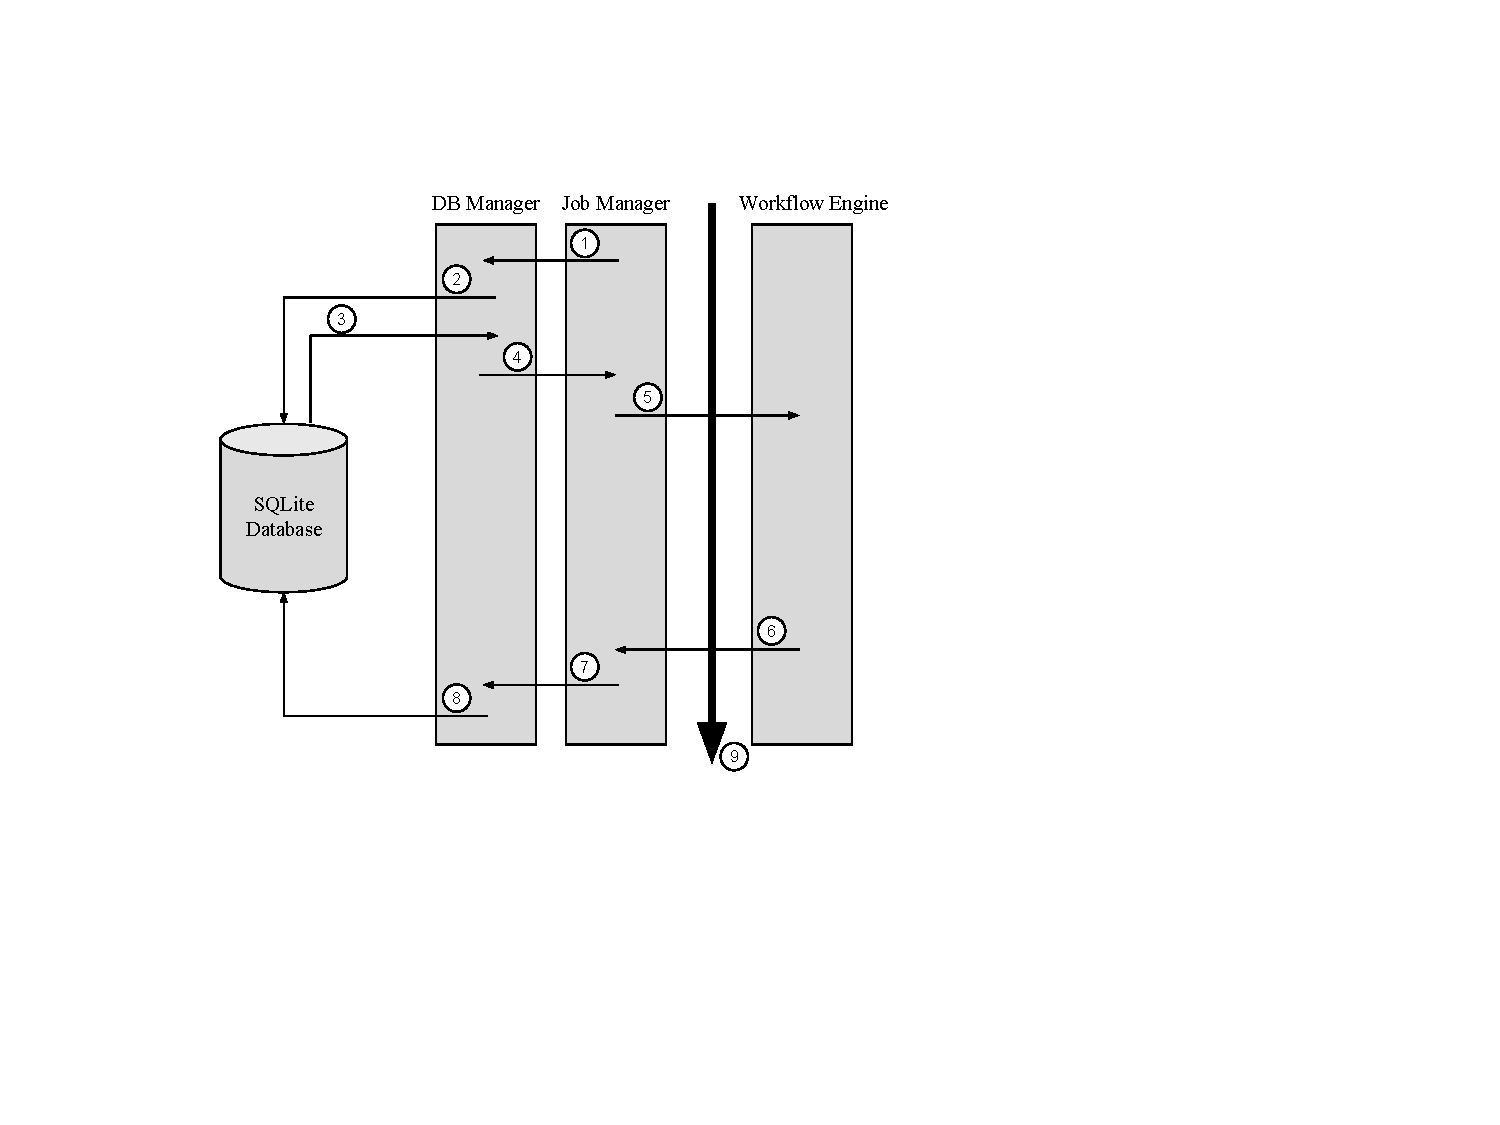
\includegraphics[width=5in]{ch-workflow/figures/WorkflowManagement.pdf}
   \caption[Steering process of the workfow management system]
   {Steering process of the workflow management system. Two objects (DB
   manager and Job Manager) serve as an interface between the database and the
   workflow engine. The job manager requests data from the DB manager~(1), which
  polls an SQLite database~(2). Once the request is served~(3), executables,
   parameters, and inputs are formatted (4) to feed the workflow engine~(5). The
   workflow engine transparently launches the job and monitors its status, which is
   then returned~(6). The status is used to update the database~(7, 8) in order
   to keep track of the inversion status. This process is repeated~(9), until
   everything has been processed.}
   \label{fig:workflow_management}
\end{figure}

For now, the workflow engine is rudimentary and relies on Radical-SAGA to launch
jobs. Adapting it to a more complete solution, similar to Ensemble-MD, is
ongoing. Relying on Radical-Pilot, patterns common to seismic inversions would
be exhibited and released to the public.

\subsection{Additional challenges}

As we progress through the implementation and the understanding of automated
seismic inversion workflows, several challenges worth mentioning will need to
be taken care of.
Taking full advantage of large-scale resources requires tight software
integration. For instance, some next generation supercomputers will have burst
buffers allowing staging of data between computing steps. While this is a promise
of greater performance, this is problematic from a workflow management
perspective. Indeed, such techniques disrupt the control flow and defy the
purpose of a workflow engine. How to solve this is an open question.
A second challenge comes from the desire of scientists to visualize intermediate
data. This is motivated by the will to take informed decisions to steer the
inversion process in the best direction possible. This calls for a level of
interactivity that interfaces well with an automated approach.

It is equally important to start thinking from the beginning about the general
geophysicist population and how they can benefit from developments made
for large-scale inversions. We are confident that the pattern defining approach
of the Ensemble toolkits, along with the system-agnostic Radical-SAGA backend,
is a step toward dissemination.
% \\
% During the first tests, our work has been carried out on a local machine with a
% personal HTCondor installation. More advanced test have been performed on a
% virtual machine running Ubuntu. This virtual machine is spawned by Vagrant,
% using Chef recipes. In the longer term this will allow seamless deployment of
% the seismic inversion workflow on a variety of computational infrastructures.
